\documentclass[a4paper,12pt]{article}
\usepackage[top = 2.5cm, bottom = 2.5cm, left = 2.5cm, right = 2.5cm]{geometry}
\usepackage[T1]{fontenc}
\usepackage[utf8]{inputenc}
\usepackage{multirow} 
\usepackage{booktabs} 
\usepackage{graphicx}
\usepackage[spanish]{babel}
\usepackage{setspace}
\setlength{\parindent}{0in}
\usepackage{float}
\usepackage{fancyhdr}
\usepackage{amsmath}
\usepackage{amssymb}
\usepackage{amsthm}
\usepackage[numbers]{natbib}
\newcommand\Mycite[1]{%
	\citeauthor{#1}~[\citeyear{#1}]}
\usepackage{graphicx}
\usepackage{subcaption}
\usepackage{booktabs}
\usepackage{etoolbox}
\usepackage{minibox}
\usepackage{hyperref}
\usepackage{xcolor}
\usepackage{pdfpages}
\usepackage[skins]{tcolorbox}
%---------------------------

\newtcolorbox{cajita}[1][]{
	 #1
}

\newenvironment{sol}
{\renewcommand\qedsymbol{$\square$}\begin{proof}[\textbf{Solución.}]}
	{\end{proof}}

\newenvironment{dem}
{\renewcommand\qedsymbol{$\blacksquare$}\begin{proof}[\textbf{Demostración.}]}
	{\end{proof}}

\newtheorem{problema}{Problema}
\newtheorem{definicion}{Definición}
\newtheorem{ejemplo}{Ejemplo}
\newtheorem{teorema}{Teorema}
\newtheorem{corolario}{Corolario}[teorema]
\newtheorem{lema}[teorema]{Lema}
\newtheorem{prop}{Proposición}
\newtheorem*{nota}{\textbf{NOTA}}
\renewcommand\qedsymbol{$\blacksquare$}
\usepackage{svg}
\usepackage{tikz}
\usepackage[framemethod=default]{mdframed}
\global\mdfdefinestyle{exampledefault}{%
linecolor=lightgray,linewidth=1pt,%
leftmargin=1cm,rightmargin=1cm,
}




\newenvironment{noter}[1]{%
\mdfsetup{%
frametitle={\tikz\node[fill=white,rectangle,inner sep=0pt,outer sep=0pt]{#1};},
frametitleaboveskip=-0.5\ht\strutbox,
frametitlealignment=\raggedright
}%
\begin{mdframed}[style=exampledefault]
}{\end{mdframed}}
\newcommand{\linea}{\noindent\rule{\textwidth}{3pt}}
\newcommand{\linita}{\noindent\rule{\textwidth}{1pt}}

\AtBeginEnvironment{align}{\setcounter{equation}{0}}
\pagestyle{fancy}

\fancyhf{}









%----------------------------------------------------------
\lhead{\footnotesize Data Science I}
\rhead{\footnotesize  Rudik Roberto Rompich}
\cfoot{\footnotesize \thepage}


%--------------------------

\begin{document}
 \thispagestyle{empty} 
    \begin{tabular}{p{15.5cm}}
    \begin{tabbing}
    \textbf{Universidad del Valle de Guatemala} \\
    Departamento de Ciencias de la Computación\\\\
   \textbf{Estudiantes:} Augusto Alonso, Angel Cuellar, Rudik Roberto Rompich\\
    \end{tabbing}
    \begin{center}
        CC3066 - Data Science I - Catedrático: Luis Furlan\\
        \today
    \end{center}\\
    \hline
    \\
    \end{tabular} 
    \vspace*{0.3cm} 
    \begin{center} 
    {\Large \bf  Proyecto 2 - Análisis Exploratorio 
} 
        \vspace{2mm}
    \end{center}
    \vspace{0.4cm}
%--------------------------

\section{Análisis exploratorio}

El repositorio donde se puede encontrar el código es el siguiente: \textcolor{blue}{\href{https://github.com/RudiksChess/UVG-DataScience-Notas-6-Semestre/blob/main/Lab1/Code/Lab1.ipynb}{Github}}.

\begin{figure}[H]
	\centering 
	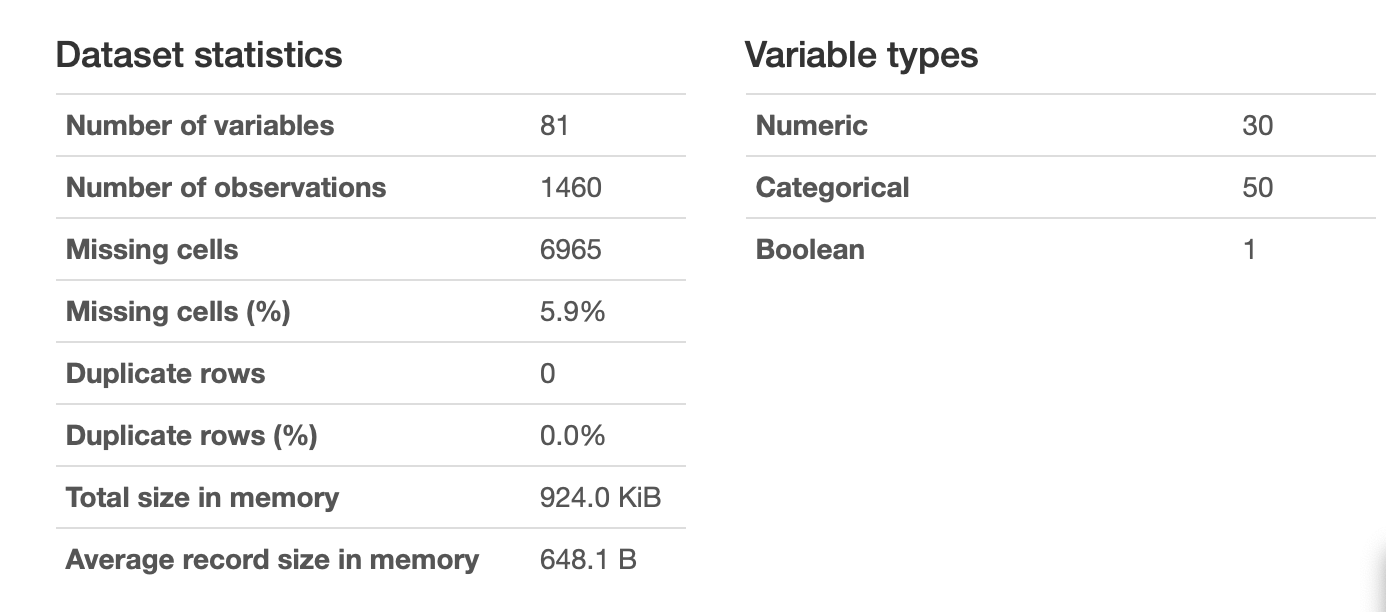
\includegraphics[scale=0.25]{Images/1}
	\caption{Resumen de la base de datos.}
	\label{fig:1}
\end{figure}

\begin{figure}[H]
	\begin{tabular}{ccc}
		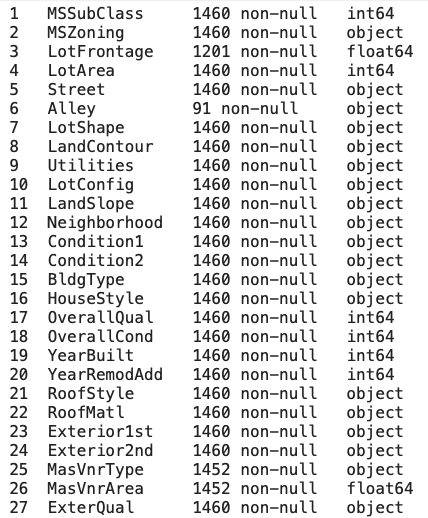
\includegraphics[width=45mm]{Images/1.1} &   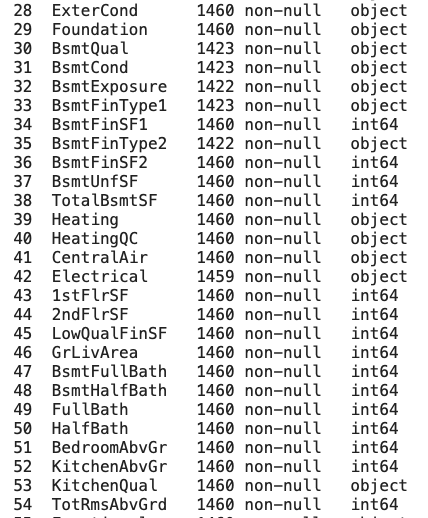
\includegraphics[width=45mm]{Images/1.2}&   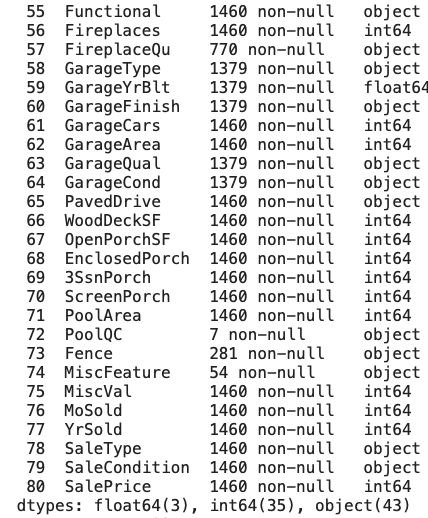
\includegraphics[width=45mm]{Images/1.3} \\
	\end{tabular}
	\caption{Clasificación de las variables.}
		\label{fig:2}
\end{figure}

\begin{figure}[H]
	\centering 
	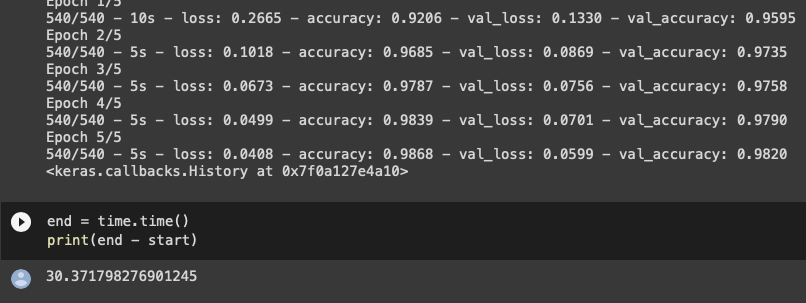
\includegraphics[scale=0.07]{Images/3}
	\caption{Gráficas de dispersión exploratoria de las variables.}
		\label{fig:3}
\end{figure}

\begin{figure}[H]
	\centering 
	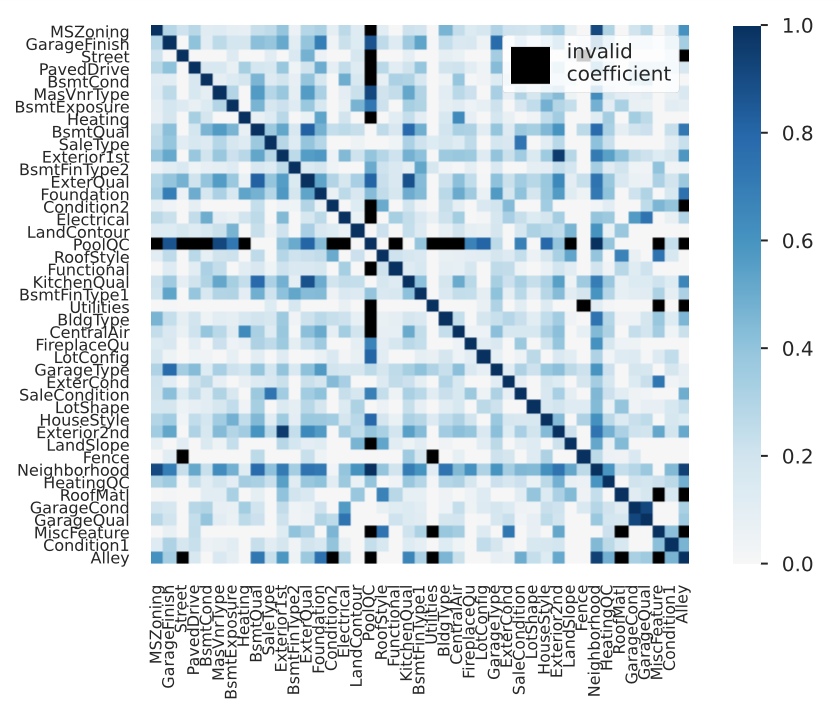
\includegraphics[scale=.4]{Images/4}
	\caption{Gráfica de correlación de Phick de variables categóricas.}
	\label{fig:4}
\end{figure}

\begin{figure}[H]
	\centering 
	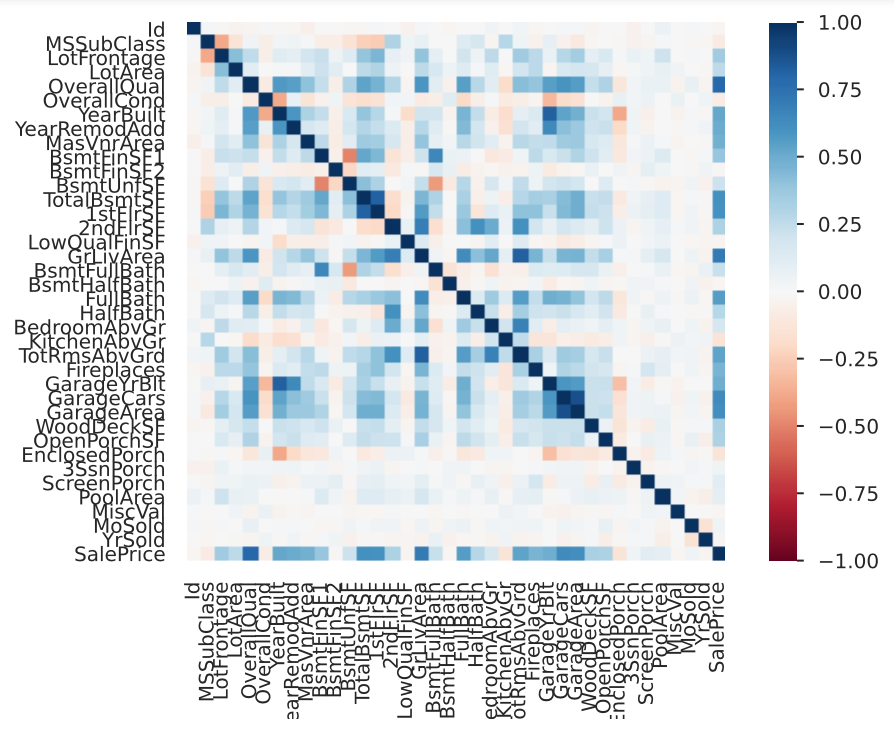
\includegraphics[scale=.4]{Images/5}
	\caption{Gráfica de correlación de Pearson de variables numéricas.}
		\label{fig:5}
\end{figure}


\begin{figure}[H]
	\centering
	\begin{tabular}{cc}
		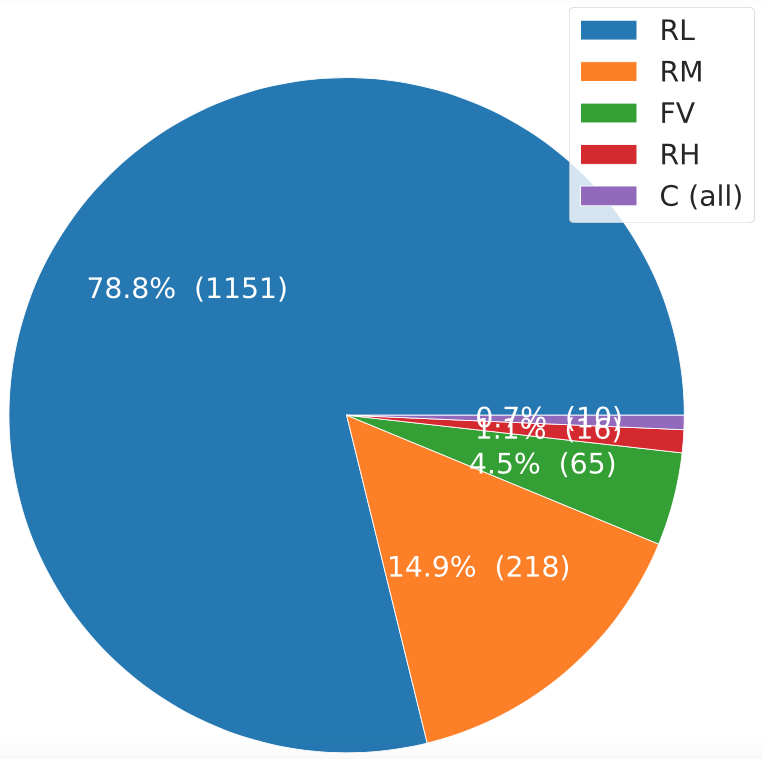
\includegraphics[width=45mm]{Images/6.1} &   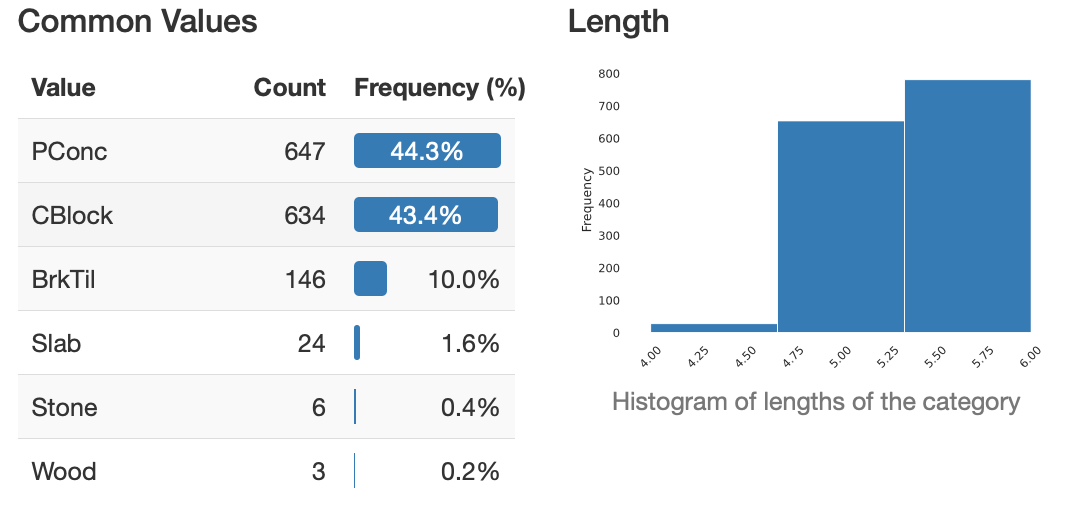
\includegraphics[width=70mm]{Images/6.2}
	\end{tabular}
	\caption{Exploración de las variables categóricas.}
		\label{fig:6}
\end{figure}

\begin{figure}[H]
	\centering
	\begin{tabular}{cc}
		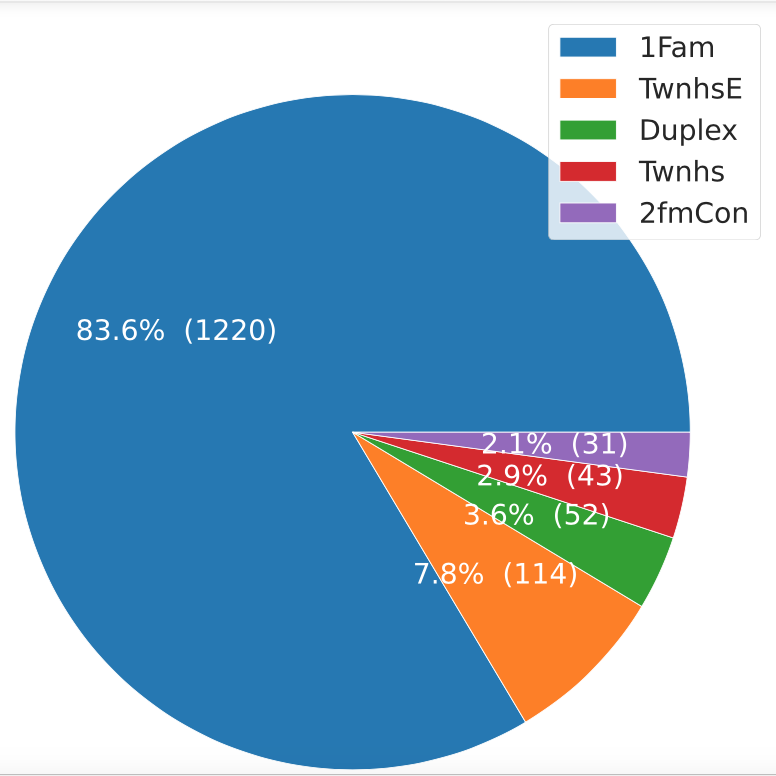
\includegraphics[width=45mm]{Images/6.3} &   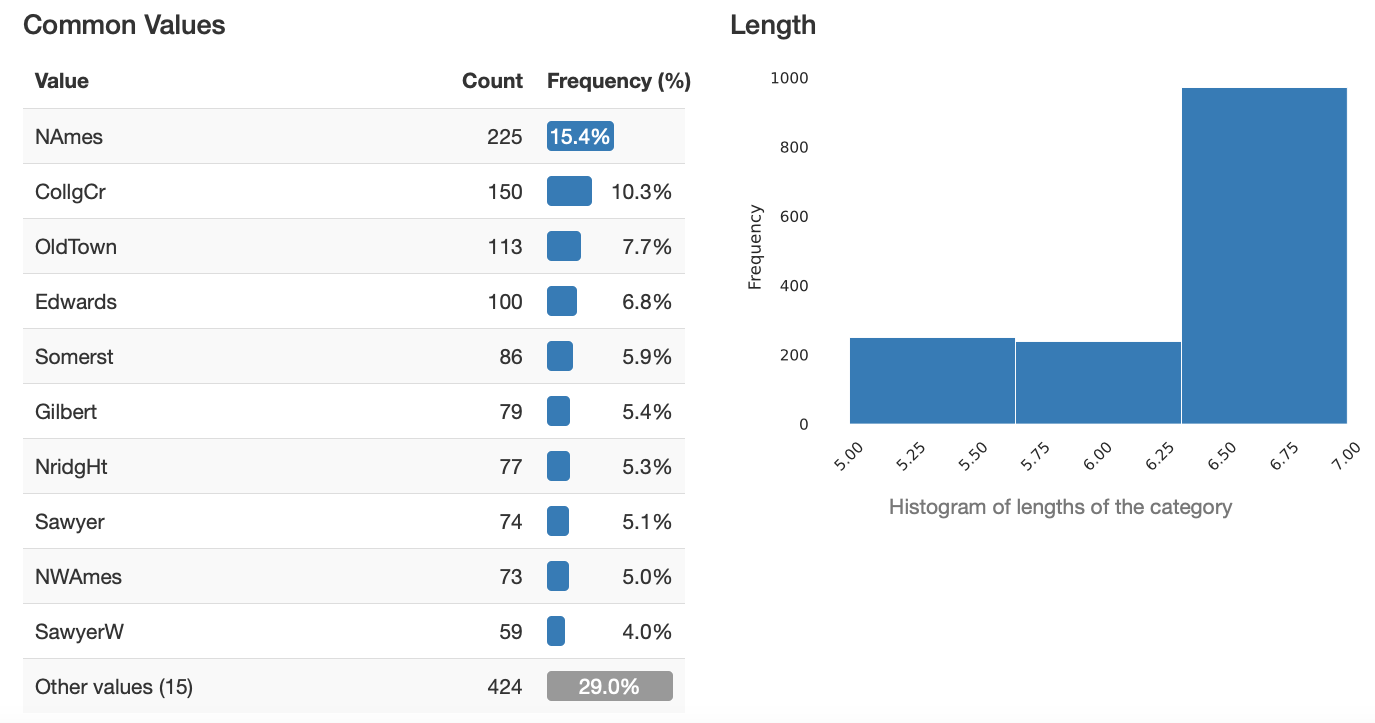
\includegraphics[width=70mm]{Images/6.4}
	\end{tabular}
	\caption{Exploración de las variables categóricas.}
		\label{fig:7}
\end{figure}


\begin{figure}[H]
	\centering
	\begin{tabular}{cc}
		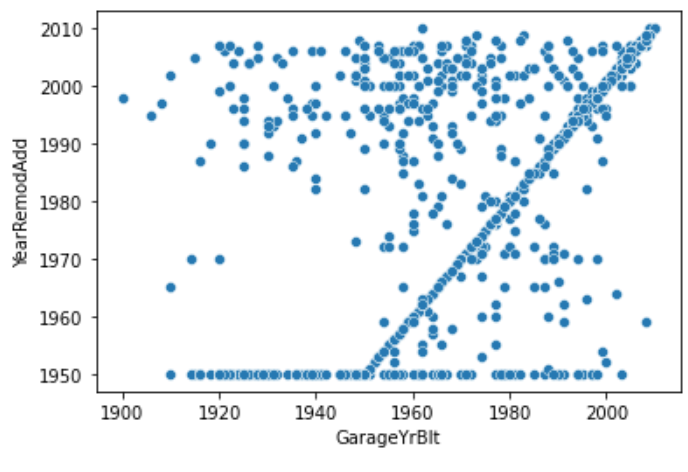
\includegraphics[width=45mm]{Images/7} &   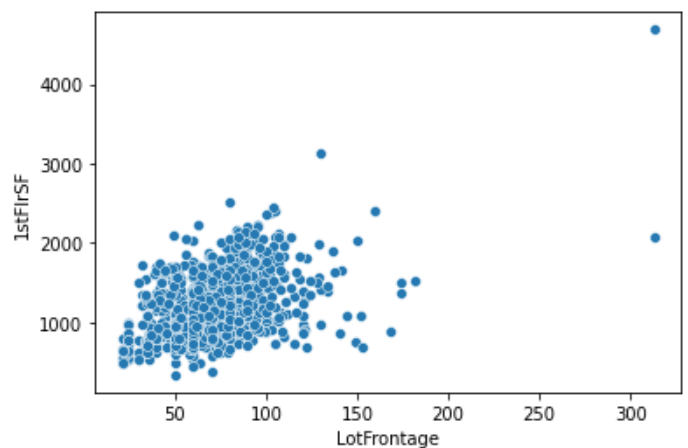
\includegraphics[width=45mm]{Images/7.1}
	\end{tabular}
	\caption{Exploración de las variables numéricas.}
		\label{fig:8}
\end{figure}

\begin{figure}[H]
	\centering
	\begin{tabular}{cc}
		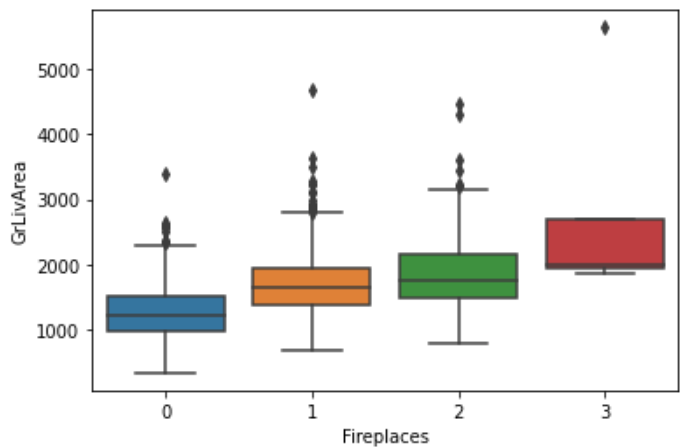
\includegraphics[width=45mm]{Images/7.2} &   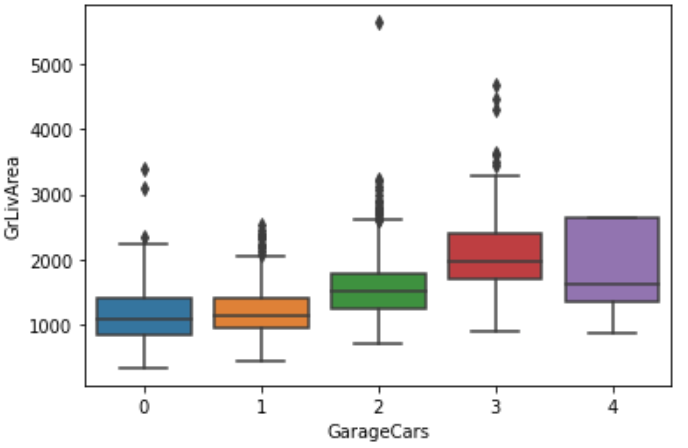
\includegraphics[width=45mm]{Images/7.3}
	\end{tabular}
	\caption{Exploración de las variables numéricas.}
		\label{fig:9}
\end{figure}


\newpage 


\begin{cajita}
	Las siguientes dos secciones no fueron requeridas en este laboratorio:
	\begin{enumerate}
		\item Análisis de Componente Principales
		\item Reglas de Asociación
	\end{enumerate}
\end{cajita}


\section{Hallazgos y Conclusiones}

Para la mayoría de incisos de este ejercicio se usó el \textbf{Pandas Profiler}. 

\subsection{Variables}

Un análisis preliminar de clasificación de los tipos de variables con \textbf{Pandas Profiler} \ref{fig:1} arroja que existen 30 variables numéricas, 50 variables categóricas y 1 variable booleana que podría considerarse como categórica también. Por otra parte, un análisis más rudimentario \ref{fig:2} arroja que existen: 
\begin{enumerate}
	\item $float64$ tiene 3 variables, estas variables se podrían considerar \textit{variables cuantitativas continuas}. 
	\item $int64$ tiene 35 variables, estas variables se podrían considerar \textit{variables cuantitativas discretas}. Excluyendo las variables que contengan años, estas podrían tomarse como \textit{variables categóricas}.  
	\item $object$ tiene 43 variables, estas variables se podrían considerar \textit{variables categóricas o cualitativas}.
\end{enumerate}

\begin{cajita}
	La interpretación precisa de cada de una de las variables es un proceso no automatizado y por lo tanto, las variables como los años se podrían tomar como categóricas según sea el problema que se trata. 
\end{cajita}

\subsection{Gráficos exploratorios}

Una gráfica de dispersión preliminar de las relaciones entre las 81 variables \ref{fig:3} muestran una gran variedad de relaciones y dispersiones del conjunto dado. 

\subsection{Correlación}

Para la exploración de correlación de las variables categóricas se utilizó la correlación de Phick \ref{fig:4} y para las variables numéricos la correlación de Pearson \ref{fig:5}. Cuando la correlación es muy alta, los valores se asemejan a un color más cercano al azul oscuro, como se indica en el cuadro lateral de las correlaciones. 


\subsection{Variables categóricas}

En \ref{fig:6} y \ref{fig:1} se ofrecen algunas gráficas relacionadas a las variables categóricas. Existen distintos tipos de relaciones que se pueden observar a mayor profundidad en el pandas profiler que adjunta en el código. 

\subsection{Variables numéricas}
En \ref{fig:8} y \ref{fig:9} se ofrecen algunas gráficas relacionadas a las variables categóricas. Existen distintos tipos de relaciones que se pueden observar a mayor profundidad en el pandas profiler que se adjunta en el código. 



\section{Conclusión}

Existen una gran diversidad de relaciones con los datos proporcionados; algunas columnas tienen muchas datos nulos; por lo tanto, sería necesario eliminarlos, ya que no aportarían nada a un futuro modelo. 



%---------------------------
%\bibliographystyle{apa}
%\bibliography{referencias.bib}

\end{document}